% Created 2023-01-30 Mon 07:54
% Intended LaTeX compiler: lualatex
\documentclass[bigger]{beamer}
\usepackage{graphicx}
\usepackage{longtable}
\usepackage{wrapfig}
\usepackage{rotating}
\usepackage[normalem]{ulem}
\usepackage{amsmath}
\usepackage{amssymb}
\usepackage{capt-of}
\usepackage{hyperref}
\usetheme[progressbar=foot, sectionpage=none, numbering=fraction]{metropolis}
\usepackage{tikz}
\usepackage{booktabs}
\usepackage{adjustbox}
\usepackage{diagbox}
\usepackage{latexcolors}
\usetikzlibrary{automata, positioning, arrows, arrows.meta}
\usepackage{diagbox}
\usepackage{dsfont}
\usepackage{amsmath}
\usepackage{fontawesome5}
\definecolor{RedBrown}{RGB}{192, 4, 4} \setbeamercolor{progress bar}{fg=RedBrown} \setbeamercolor{title separator}{fg=RedBrown}
\setbeamercolor{progress bar in head/foot}{fg=RedBrown} \setbeamercolor{progress bar in section page}{fg=RedBrown} \setbeamercolor{alerted text}{fg=RedBrown}
\pretocmd{\tableofcontents}{\thispagestyle{empty}}{}{}
\addtocounter{framenumber}{-1}
\usepackage{listings}
\usepackage{xcolor}
\definecolor{codegreen}{rgb}{0,0.6,0}
\definecolor{codegray}{rgb}{0.5,0.5,0.5}
\definecolor{codepurple}{rgb}{0.58,0,0.82}
\definecolor{backcolour}{HTML}{f0f0f0}
\lstdefinestyle{mystyle}{
backgroundcolor=\color{backcolour},
commentstyle=\color{codegreen},
keywordstyle=\color{magenta},
numberstyle=\tiny\color{codegray},
stringstyle=\color{codepurple},
basicstyle=\ttfamily,
breakatwhitespace=false,
breaklines=true,
captionpos=b,
keepspaces=true,
numbers=none,
numbersep=5pt,
showspaces=false,
showstringspaces=false,
showtabs=false,
tabsize=2
}
\lstset{style=mystyle}
\usetheme{default}
\author{Andrea Pierré}
\date{January 30\textsuperscript{th}, 2023}
\title{Joint RL meeting}
\subtitle{Gridworld implementation of Olivia's task}
\institute{Brown University}
\titlegraphic{\hfill
\includegraphics[height=1.5cm]{img/Brown Logo_2016_2 Color Process ST_1300.png}}
\setbeamercovered{transparent=10}
\setbeamertemplate{section in toc}[sections numbered]
\AtBeginSection[]{\begin{frame}[plain, noframenumbering]{Outline}    \setbeamertemplate{section in toc}[sections numbered]\setbeamertemplate{subsection in toc}[subsections numbered]\vspace{-0.8em}\tableofcontents[currentsection, currentsubsection]\end{frame}}
\AtBeginSubsection[]{\begin{frame}[plain, noframenumbering]{Outline}\setbeamertemplate{section in toc}[sections numbered]\setbeamertemplate{subsection in toc}[subsections numbered]\tableofcontents[currentsection,currentsubsection]\end{frame}}
\hypersetup{
 pdfauthor={Andrea Pierré},
 pdftitle={Joint RL meeting},
 pdfkeywords={},
 pdfsubject={},
 pdfcreator={Emacs 28.2 (Org mode 9.6)}, 
 pdflang={English}}
\begin{document}

\maketitle
\begin{frame}{Outline}
\tableofcontents
\end{frame}

\section{Implementation}
\label{sec:org9dde8a0}
\begin{frame}[<+->][label={sec:orgf5dedb6},fragile]{Implementation}
 \begin{itemize}
\item RL concepts abstracted in high level functions :
\begin{itemize}
\item \texttt{reset()}: reset the environment at the end of the episode
\item \texttt{reward()}: define in what conditions the agent get a reward and how much reward it gets
\item \texttt{is\_terminated()}: define when the end of the episode has been reached
\item \texttt{step()}: execute the defined action in the current state
\scriptsize
\begin{lstlisting}[language={Python}]
new_state, reward, done = env.step(action, state)
\end{lstlisting}
\end{itemize}
\end{itemize}
\end{frame}
\begin{frame}[<+->][label={sec:org2276fa8}]{Implementation}
\begin{itemize}
\item At each step, the agent gets a composite observation:
\end{itemize}
\begin{center}
\begin{tabular}{ll}
\hline
location & cue\\
\hline
\{0,\ldots{},24\} & North light\\
 & South light\\
 & Odor A\\
 & Odor B\\
\hline
\end{tabular}
\end{center}
\begin{itemize}
\item Convenience functions to translate the movements between the grid positions and the states
\end{itemize}
\end{frame}
\begin{frame}[<+->][label={sec:orgf3b191f},fragile]{Implementation}
\begin{itemize}
\item Wrapper environment to translate the human readable environment (\alert{composite states}) into a suitable environment for the Q-learning algorithm (\alert{flat states})
\scriptsize
\begin{lstlisting}[language={Python}]
state = {"location": 13, "cue": LightCues.South}
env.convert_composite_to_flat_state(state)
# => 38
\end{lstlisting}
\begin{lstlisting}[language={Python}]
state = 63
env.convert_flat_state_to_composite(state)
# => {"location": 13, "cue": <OdorID.A: 1>}
\end{lstlisting}
\item Human readable objects
\scriptsize
\begin{lstlisting}[language={Python}]
action = 0
Actions(action).name
# => "UP"
\end{lstlisting}
\end{itemize}
\end{frame}
\section{Issues along the road}
\label{sec:orgd24dc37}
\begin{frame}[label={sec:org8bcff10}]{Not enough states to solve the task}
\begin{columns}
\begin{column}{0.45\columnwidth}
\begin{center}
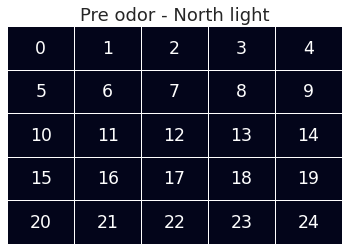
\includegraphics[width=.9\linewidth]{img/state_space_1.png}
\end{center}
\begin{center}
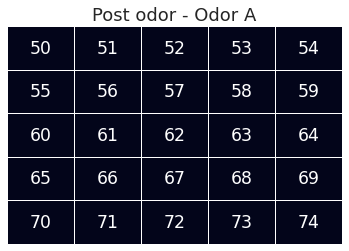
\includegraphics[width=.9\linewidth]{img/state_space_3.png}
\end{center}
\end{column}
\begin{column}{0.45\columnwidth}
\begin{center}
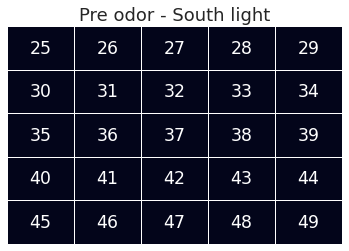
\includegraphics[width=.9\linewidth]{img/state_space_2.png}
\end{center}
\begin{center}
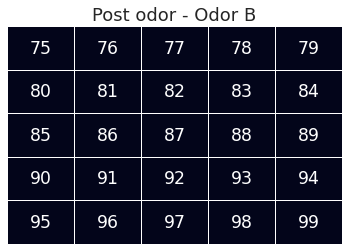
\includegraphics[width=.9\linewidth]{img/state_space_4.png}
\end{center}
\end{column}
\end{columns}
\end{frame}
\begin{frame}[label={sec:orgbcda695}]{\(\epsilon\)-greedy when Q-values are identical}
\begin{columns}
\begin{column}{0.5\columnwidth}
\centering
Vanilla \epsilon-greedy\\[2em]
\begin{center}
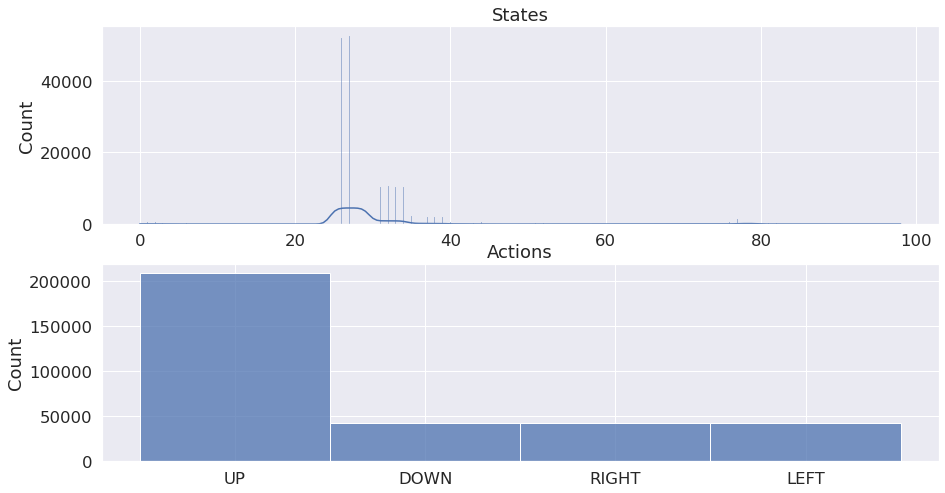
\includegraphics[width=\textwidth]{img/hist_before.png}
\end{center}
\end{column}
\begin{column}{0.5\columnwidth}
\centering
Randomly choosing actions with the same Q-values
\begin{center}
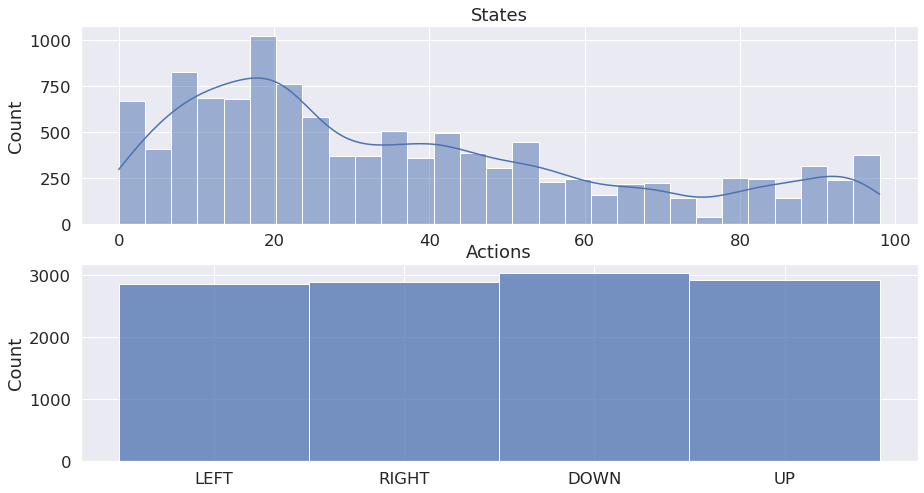
\includegraphics[width=\textwidth]{img/hist_after.png}
\end{center}
\end{column}
\end{columns}
\end{frame}
\section{Results}
\label{sec:orge88a259}
\begin{frame}[label={sec:org7e2e6cc}]{Standard Q-learning -- allocentric environment}
\begin{center}
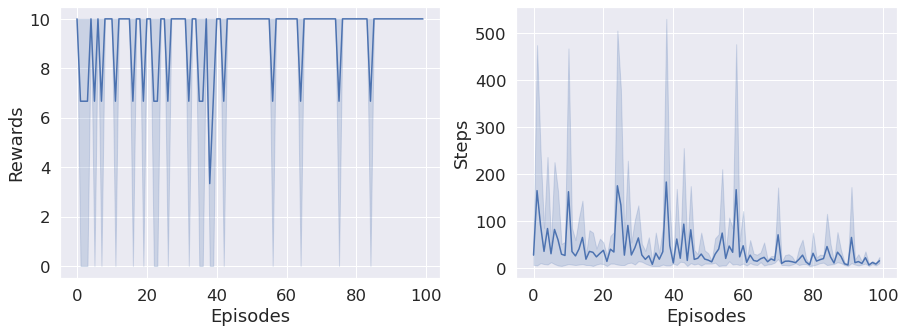
\includegraphics[width=.9\linewidth]{img/q-learning_allo_steps_rewards.png}
\end{center}
\end{frame}
\begin{frame}[label={sec:orgb202c99}]{Standard Q-learning -- allocentric environment}
\begin{center}
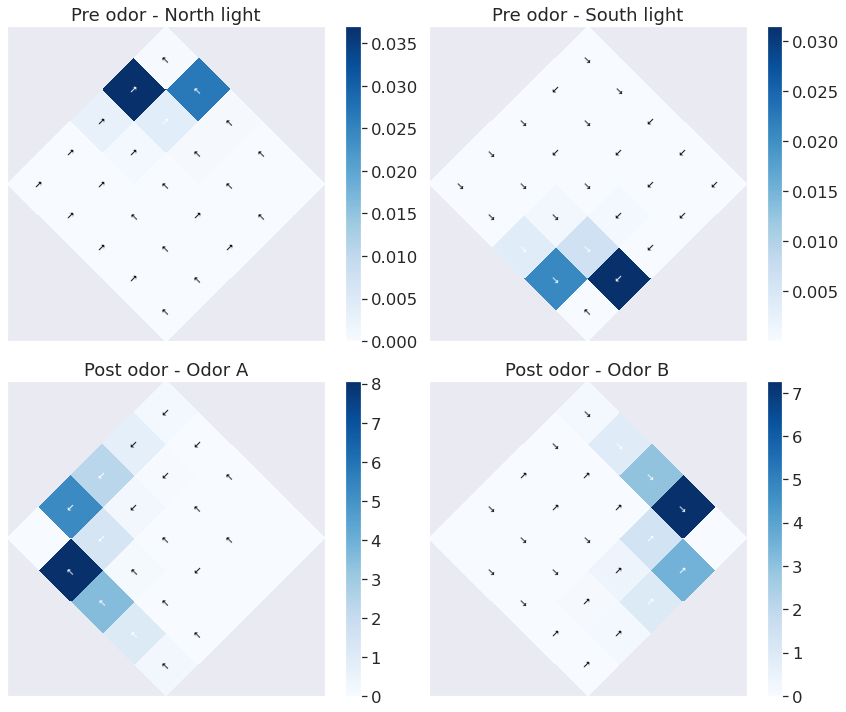
\includegraphics[width=.9\linewidth]{img/q-learning_allo_best_actions_maps.png}
\end{center}
\end{frame}
\begin{frame}[label={sec:org4581df7}]{Q-learning with function approximation -- allocentric environment -- without joint representation}
\begin{columns}
\begin{column}{0.5\columnwidth}
\begin{center}
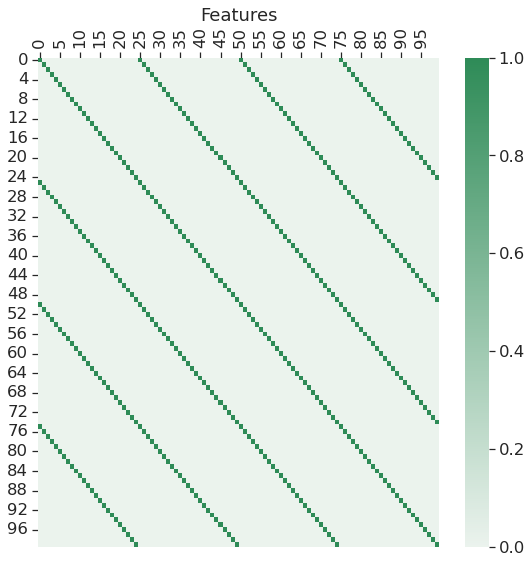
\includegraphics[height=0.4\textheight]{img/func_approx_allo_features_heatmap_nojointrep.png}
\end{center}
\end{column}
\begin{column}{0.5\columnwidth}
\begin{center}
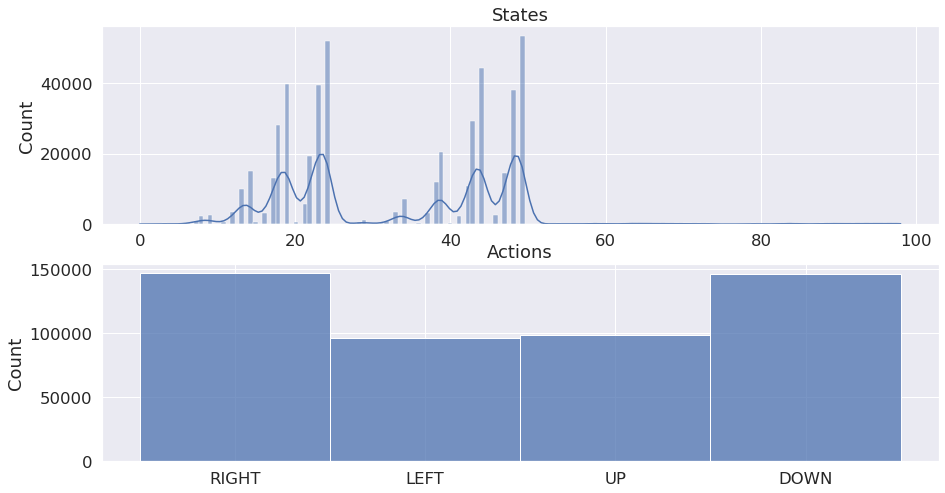
\includegraphics[width=\textwidth]{img/func_approx_allo_actions_states_hist_nojointrep.png}
\end{center}
\end{column}
\end{columns}
\begin{block}{~}
\vspace{-2em}
\begin{center}
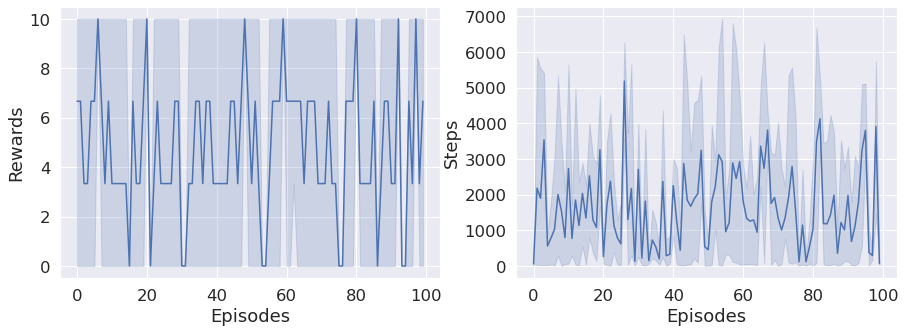
\includegraphics[height=0.4\textheight]{img/func_approx_allo_steps_rewards_nojointrep.png}
\end{center}
\end{block}
\end{frame}
\begin{frame}[label={sec:org7b17c51}]{Q-learning with function approximation -- allocentric environment -- without joint representation}
\begin{center}
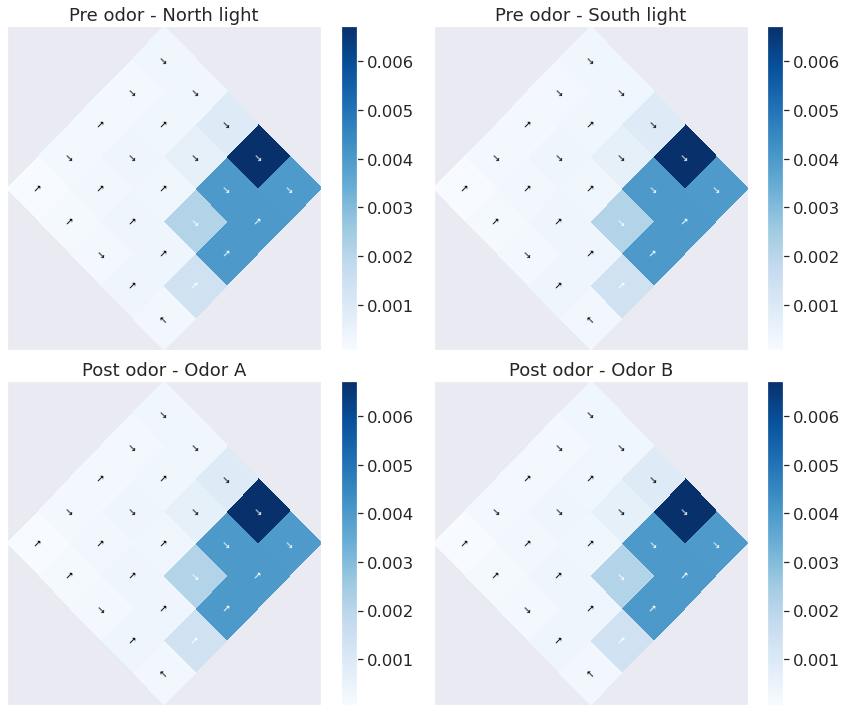
\includegraphics[height=0.8\textheight]{img/func_approx_allo_best_actions_maps_nojointrep.png}
\end{center}
\end{frame}
\begin{frame}[label={sec:orgcc2e675}]{Q-learning with function approximation -- allocentric environment -- with joint representation}
\begin{columns}
\begin{column}{0.5\columnwidth}
\begin{center}
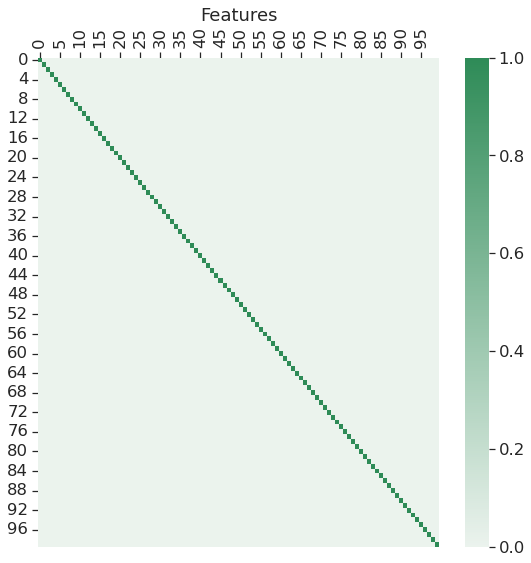
\includegraphics[height=0.4\textheight]{img/func_approx_allo_features_heatmap_jointrep.png}
\end{center}
\end{column}
\begin{column}{0.5\columnwidth}
\begin{center}
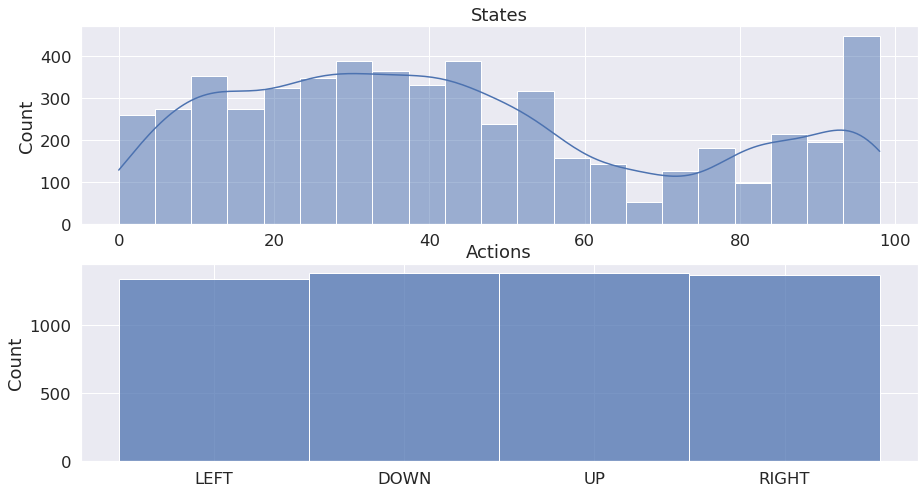
\includegraphics[width=\textwidth]{img/func_approx_allo_actions_states_hist_jointrep.png}
\end{center}
\end{column}
\end{columns}
\begin{block}{~}
\vspace{-2em}
\begin{center}
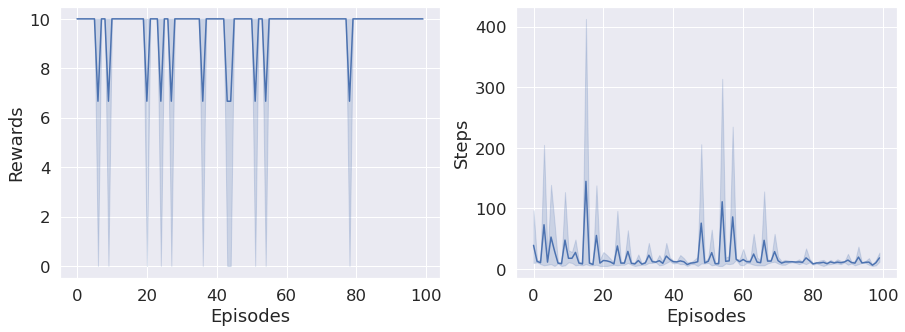
\includegraphics[height=0.4\textheight]{img/func_approx_allo_steps_rewards_jointrep.png}
\end{center}
\end{block}
\end{frame}
\begin{frame}[label={sec:org4689dfd}]{Q-learning with function approximation -- allocentric environment -- with joint representation}
\begin{center}
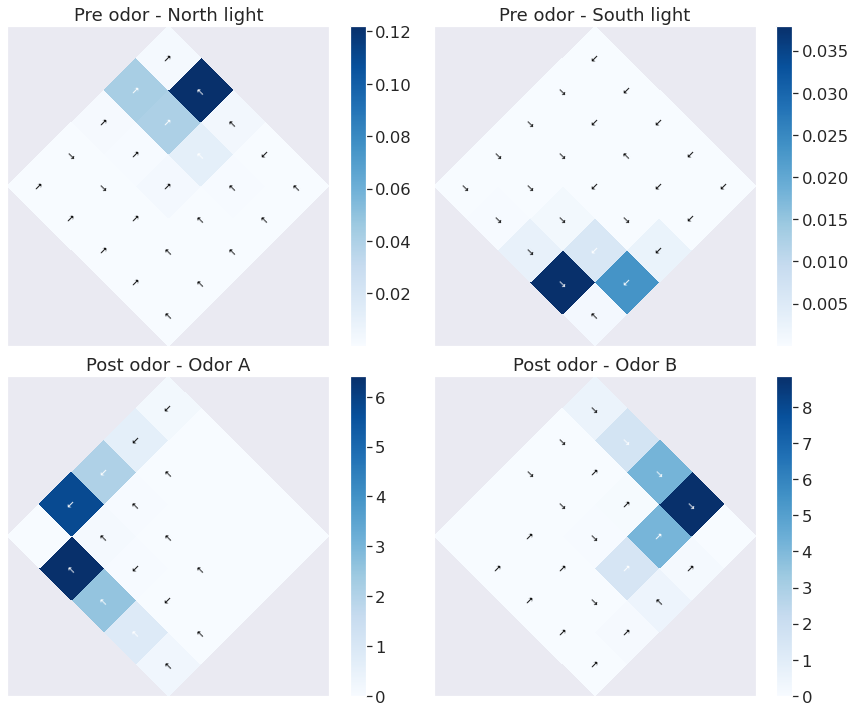
\includegraphics[height=0.8\textheight]{img/func_approx_allo_best_actions_maps_jointrep.png}
\end{center}
\end{frame}

\begin{frame}[label={sec:orgb2d6106}]{Standard Q-learning -- egocentric environment}
\begin{center}
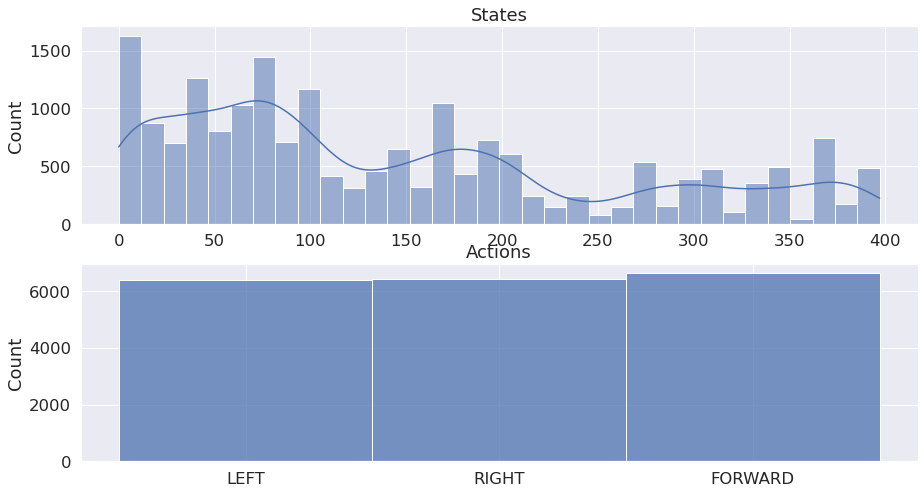
\includegraphics[height=0.4\textheight]{img/q-learning_ego_hist.png}
\end{center}
\begin{center}
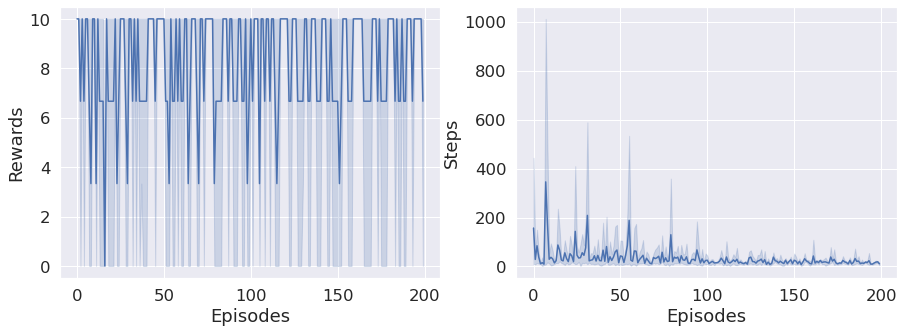
\includegraphics[height=0.4\textheight]{img/q-learning_ego_steps_rewards.png}
\end{center}
\end{frame}
\begin{frame}[label={sec:orgaa35299}]{Q-learning with function approximation -- egocentric environment}
\begin{center}

\includegraphics[height=0.5\textheight]{img/work-in-progress.png}
\end{center}
\end{frame}

\section{Summary}
\label{sec:org2290226}
\begin{frame}[<+->][label={sec:orga01e917}]{Summary}
\begin{itemize}
\item Standard Q-learning can learn the task in the \alert{allocentric} environment in \textasciitilde{}50 episodes
\item Standard Q-learning can learn the task in the \alert{egocentric} environment in \textasciitilde{}100 episodes
\item Niloufar's results with function approximation on the allocentric environment are reproducible :
\begin{itemize}
\item The agent is \alert{not able to learn} the task \alert{without} having a place-odor joint representation
\item \alert{With} a place-odor joint representation, the agent is \alert{able to learn the task} in \textasciitilde{}60 episodes
\end{itemize}
\end{itemize}
\end{frame}
\begin{frame}[label={sec:org7f179d0}]{Main differences with Niloufar's model}
\begin{columns}
\begin{column}{0.7\columnwidth}
\begin{itemize}
\item The environment is \alert{closer to the real experiment} \(\to\)~ports are in the corners of the arena, not in the middle of the walls
\item Code is clean, readable, and abstracted in high level functions/concepts
\end{itemize}
\end{column}
\begin{column}{0.3\columnwidth}
\begin{center}
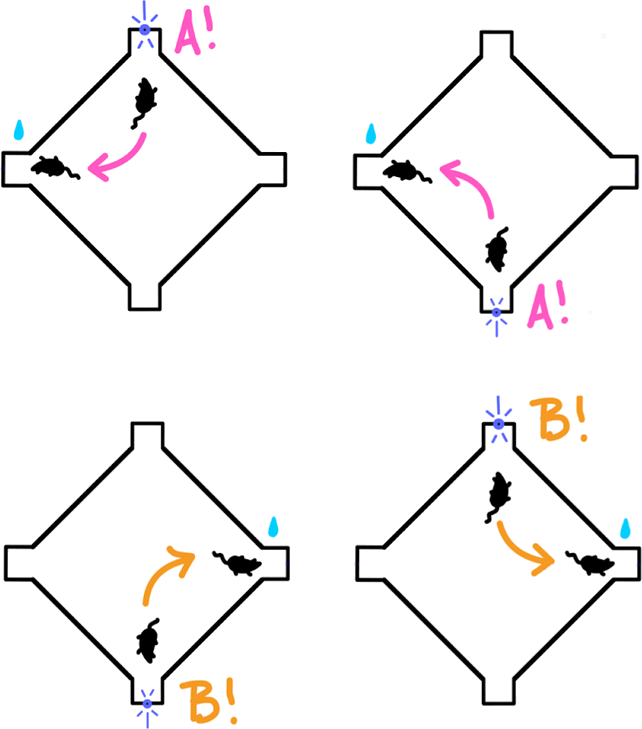
\includegraphics[width=\textwidth]{img/task.png}
\end{center}
\begin{center}
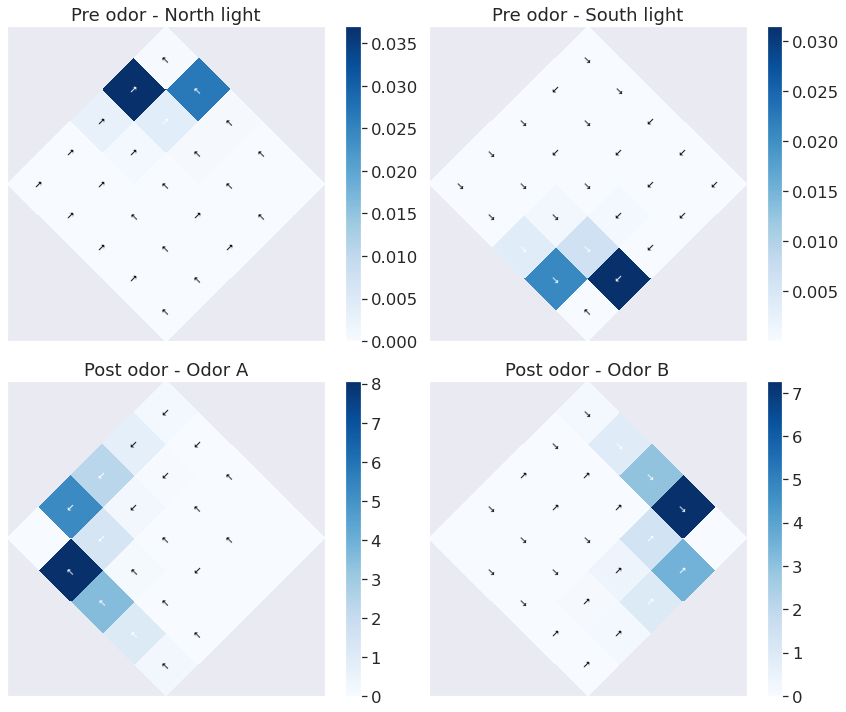
\includegraphics[width=\textwidth]{img/q-learning_allo_best_actions_maps.png}
\end{center}
\end{column}
\end{columns}
\end{frame}
\begin{frame}[<+->][label={sec:org56f0e23}]{Next steps}
\begin{itemize}
\item Finish the egocentric environment
\item Replace the manually crafted features matrix by an artificial neural network, which should learn the necessary representations to solve the task from scratch
\end{itemize}
\end{frame}
\begin{frame}[label={sec:org2220530},standout]{~}
Questions ?
\end{frame}
\end{document}
